\definecolor{customblue}{HTML}{155DFC}

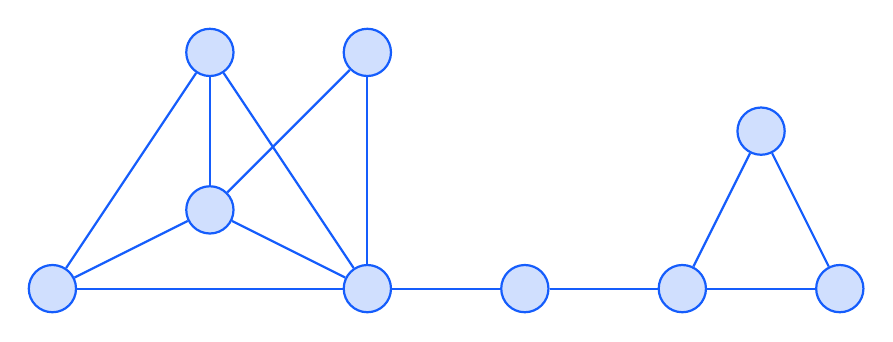
\begin{tikzpicture}[scale=1,auto=left,every node/.style={circle,fill=customblue!20,draw=customblue,thick,minimum size=6mm}]
  \node (n1) at (0,0) {};
  \node (n2) at (2,3) {};
  \node (n3) at (2,1) {};
  \node (n4) at (4,3) {};
  \node (n5) at (4,0) {};
  \node (n6) at (6,0) {};
  \node (n7) at (8,0) {};
  \node (n8) at (9,2) {};
  \node (n9) at (10,0) {};
  \foreach \from/\to in {n1/n2,n1/n3,n1/n5,n2/n3,n2/n5,n3/n4,n3/n5,n4/n5,n5/n6,n6/n7,n7/n8,n7/n9,n8/n9}
    \draw[customblue,thick] (\from) -- (\to);
\end{tikzpicture}
